\documentclass[main]{subfiles}

\begin{document}
% Chapter Template
\setcounter{chapter}{1}

% Evolutionary Optimization
% Basic components
%  Universe, Planets and Environments
%   Planet Physics
%  Epochs
%   Fitness functions
%  Populations
%  Creatures
%   Genotypes
%   Phenotypes
%    Constrained Rigid body model
%    Featherstone Multi-rigidbody model
%  Model organisms
% Reaper
%  Crossover
%  Mutations
% Evaluation Step
% Variation Step
\chapter{Evolutionary Optimization} % Main chapter title

\label{Chapter\thechapter} % Change X to a consecutive number; for referencing this chapter elsewhere, use \ref{ChapterX}

\lhead{Chapter \thechapter. \emph{Evolutionary Optimization}} % Change X to a consecutive number; this is for the header on each page - perhaps a shortened title

The following chapter describes the evolutionary optimization algorithm as it is implemented in the Minemonics simulator. The Minemonics simulator is the experimentation platform used throughout this Thesis and is a project that was developed from scratch, mainly because other simulators for evolving virtual creatures are unpublished by the respective research groups, are outdated or implement a different type of simulation than is needed for the model of this Thesis. Apart from the research interests, the simulator was made to be extensible for other research experiments to be implemented. It is available open-source from its git repository on github [?].

\section{Basic components}
% rev. 1

To understand the purpose of the simulation, it is important to first understand the different basic components of it. Therefore, we first discuss the basic components of the simulator and their respective features. The tree of components is described in a top-down manner and the subcomponents are revealed one-by-one to start out simple and slowly reveal complexity. 

%-----------------------------------
%	SUBSECTION 1
%-----------------------------------
\subsection{Universe, Planets and Environments}
% rev. 1

The main model of the simulation is its own universe. The simulator's universe is a set of different planets, each planet being a certain setting of evolutionary run. A certain planet consists of an environment, an instance of evolutionary process and a number of epochs. 

The environment is a representation of a flat plane or a hill environment. For the experiments in this thesis, mainly the plane environment was used.

The type of evolutionary process instance defines how many creatures of the planet are evaluated simultaneously in the same environment and the percentage of creatures that are culled, variated and sown. Within the bounds of this thesis, only single creature evaluation was performed. 

\subsubsection{Planet physics}
% rev. 1

Each environment defines the type of planet physics simulation. The two types of environments currently available, flat plane and hill environment, both simulate the environment and the creatures using newtonian mechanical physics. To do that, the simulator uses the Bullet Physics engine\cite{bulletphysics} to build a terrain for the creatures to move upon and builds the creatures using different rigid body primitive types such as boxes or cones which are held together by joint constraints with different configurations. Bullet Physics is a numerical classical mechanics simulation engine, featuring rigid body as well as soft body physics. Bodies can be constrained using various types of constraints with constraint limits and motors. The constraints are numerically solved using one of the many types of available solvers with different convergence speeds and accuracy of result. The most robust results were achieved using the Featherstone Multibody solver. To date it only supports single degree of freedom joints, however this does not affect the evolutionary optimization much. A three degrees of freedom joint can easily be approximated by three one degree of freedom joints.

\subsection{Epochs}
% rev. 1

An epoch of a certain planet models the changes of environmental factors, which induce modification to the fitness landscape on the planet. What is considered good in one epoch might not be good in another. The change of the fitness landscape usually leads to avalanches of extinction[?], because the changing fitness only leaves little chance for the highly adapted creature to adapt to the new conditions. In the simulation, an epoch  is represented by a set of juries(fitness functions) and a transition condition, which, when met, ends the epoch and starts the next epoch.

\subsubsection{Juries}
% rev. 2

Juries or fitness functions are part of an epoch in which they are relevant. A jury collects data on a certain performance during the evaluation of a creature and finally has to rate the performance. Commonly used juries of the simulator are the distance travelled during the evaluation time or the average height above ground of all limbs during the evaluation. A jury additionally has a combination weight, which indicates the weight of this performance in the total performance of the creature, and a sorting direction, which indicates whether a higher rating is considered better or worse than a lower rating for this type of fitness. Fitness values of different types of juries are then combined as a weighted sum based on the type-specific competitive ranking among the creatures of one population. This procedure will be described in the section \ref{subsubsection:Culling} Culling of the Reaper component.

\subsection{Populations}
\label{subsec:populations}
% rev. 2

A population of creatures in the simulator lives on a certain planet. Depending on the evolution settings of the planet, one creature, multiple creatures of one population, multiple creatures of multiple populations or multiple whole populations are evaluated at the same time within one evaluation slot. When a population is initialized, it has a certain initial number of individuals. The individuals can be completely randomly generated creatures or model organisms, the latter being common morphology primitives for testing. During the evaluation of a population, the number of individuals falls generally below the original population size, because several individuals are culled during the evaluation. This happens when creatures surpass boundaries of physical realism (a main source of this is when creatures generate high forces that lead to very fast limb velocity, leading to imaginary forces that lift creatures off the ground and make them fly), therefore the simulation culls them early to be not considered any more.

\subsection{Creatures}
% rev. 2

A creature or individual is part of a population and is subject to evaluation. The creature is based on two main components, its genotype and its phenotype. The genotype is the compact blueprint of the creature. Developed from it is the phenotype, which is the explicit form of the creature representing the body of the creature in the physics engine and the controller in its fully wired form. Furthermore we define two important measures for creatures which are its total body volume and its size. The total body volume is just the volume of all limb primitives summed up. The size of a creature \(C\) with number of limb primitives \(N(C)\) is measured as being the third root of the total volume, denoting the edge length of the total volume cube. 

\[size(C) = \sqrt[3]{\sum\limits^{N(C)}_{i=1} V(p_i)}\]

The size measure is most important because it is used to scale the fitness functions involving distances. Thereby it is possible to make a distance travelled independent of the creature size, meaning that a larger creature gets the same fitness for travelling a larger distance as a smaller creature for a smaller distance, if the ratios between creature size and respective travelled distance are the same for both creatures.

\subsubsection{Genome}
%rev. 2

In the traditional approach on genomes, a fixed length string of bits is used to encode higher order data types such as integers or doubles or into data structures such as trees or matrices. However, many state-of-the-art genomes deviate from this original representation by directly using higher order representations and thereby avoid the usually hard to solve representation problem ('What representation should be chosen so that every change in the bit string leads to a new valid representation?'). This more modern approach was also chosen in the Minemonics simulator.

The genomic model is one of the base models of the simulator. It encodes both morphology and the controller of the creature. Inspired by biological DNA, the genome of the simulator uses an indirect encoding. An indirect encoding, different from a direct encoding, does not encode every element of the phenotype explicitly, but uses element classes and branches between them to encode their relations. The advantage of indirect encodings is that an indirect coding evolves element classes instead of element instances, which leads to a higher abstraction within the genome. An element class can then be repeated several times in different scalings and symmetries, building creatures where symmetrical limbs can be evolved simultaneously.

\todo[inline]{Describe the advantage of indirect encodings over direct encodings.}

The genome defines a directed, possibly cyclic graph, where the nodes are called morphogenes, defining the classes of limbs, and where the edges are called morphogene branches, defining the joint relations inbetween the limbs. A morphogene definition (Fig. \ref{figure:genome-structure}) consists of the primitive type of the limb (a cube or capsule), the limb's dimensions, its base orientation in space, material properties such as friction, restitution and color, and a direction for the joint anchor. The joint anchor is a position on the surface of the primitive type which denotes where the parent limb will be attached through a joint in the final phenotype. Furthermore, the morphogene contains a number of morphogene branches and definitions related to how the branches are influenced by the limb. \\

A morphogene branch (Fig. \ref{figure:genome-structure}) consists of joint properties such as the pitch and yaw axis, the joint rotational limits for the pitch, yaw and roll degree of freedom, joint damping coefficients for all degrees of freedom and a controller gene.
The branch influence factors are a segment shrink factor, which shrinks all limb dimensions of the morphogene the branch points to and propagates along further branches of that morphogene.

A controller gene is either a sinusoidal controller gene or a chaotic controller gene.  The sinusoidal controller gene defines a sinusoidal controller emitting a sinusoidal signal based on x- and y-offset, a frequency and an amplitude. The sinusoidal controller is described in the section \ref{sec:sinusoidal-oscillators}. The chaotic controller gene defines a chaotic controller through the initial conditions of the system and the integration step. The chaotic controller is described in the section \ref{sec:chaotic-controllers}.

\begin{figure}[H]
\center

\begin{tikzpicture}
\pgfdeclarelayer{background}
\pgfdeclarelayer{foreground}
\pgfsetlayers{background,main,foreground}
\tikzstyle{bigbox} = [draw=black!80, thick, fill=black!5, rounded corners, rectangle]
\tikzstyle{box} = [minimum size=0.6cm, rounded corners,rectangle, fill=blue!80]

\node[align=left](1){
\underline{Genotype specification}\\
Total segment quantity limit\\
Segment tree depth limit\\
Morphogene classes vector:\\
};
\matrix(5)[below=1, row sep=2mm, column sep=2mm, inner sep=2mm] {
\node[box]{}; & \node[box]{}; & \node[box]{}; & \node[]{$\dots$}; & \node[box]{}; & \node[box]{}; & \node[box]{};\\
};

% brace to morphogene specification vector
\draw [decorate,decoration={brace,amplitude=10pt,mirror,raise=4pt},yshift=0pt]
(3.5,-2.3) -- (3.5,-0.8) node (6) [black,midway,xshift=-7cm,yshift=3.5cm] {};
%
% segment specification vector
\matrix(7)[right=6, xshift=-1.7cm,yshift=-1.5cm, row sep=2mm, column sep=2mm, inner sep=2mm] {
\node[box]{}; & \node[box]{}; & \node[box]{}; & \node[]{$\dots$}; & \node(8)[box]{}; & \node[box]{}; & \node[box]{};\\
};
%
% brach to morphogene class
\draw [decorate,decoration={brace,amplitude=10pt,mirror,raise=4pt},yshift=0pt]
(5,-2.1) -- (6.5,-2.1) node (8) [black,midway,xshift=5cm] {};
%
%
\node(9)[below=8,align=left,xshift=7cm,yshift=5.2cm]{
\underline{Morphogene class}\\
Primitive type\\
Dimensions: X, Y, Z\\
Orientation: W, X, Y, Z \\
Material properties:\\
~~Restitution\\
~~Friction\\
~~Color: R, G, B \\
Joint Anchor: X, Y, Z\\
Segment Shrink Factor\\
Repetition Limit\\
Follow-up gene\\
Morphogene branch vector:\\
};
\matrix(10)[below=9,xshift=7.5cm,yshift=-1.4cm, row sep=2mm, column sep=2mm, inner sep=2mm] {
\node[box]{}; & \node[box]{}; & \node[box]{}; & \node[]{$\dots$}; & \node[box]{}; & \node[box]{}; & \node[box]{};\\
};
%
%
\draw [decorate,decoration={brace,amplitude=10pt,mirror,raise=4pt},yshift=0pt]
(4,-10.5) -- (4,-12.1) node (11) [black,midway,xshift=7cm,yshift=-0.8cm] {};
%
%
\matrix(12)[left=11, xshift=14cm,yshift=-11.3cm, row sep=2mm, column sep=2mm, inner sep=2mm] {
\node[box]{}; & \node[box]{}; & \node[box]{}; & \node[]{$\dots$}; & \node(8)[box]{}; & \node[box]{}; & \node[box]{};\\
};
%
% brace to morphogene branch specification
\draw [decorate,decoration={brace,amplitude=10pt,mirror,raise=4pt},yshift=0pt]
(1.5,-10.7) -- (0,-10.7) node (13) [black,midway,xshift=-4cm] {};
%
%
\node[above=12,xshift=0cm,yshift=-22cm,align=left](14){
\underline{Morphogene branch specification}\\
Flipped, Mirrored \\
Joint specification:\\
~~Joint Anchor: X, Y, Z\\
~~Pitch Axis: X, Y, Z\\
~~Yaw Axis: X, Y, Z\\
~~Pitch Limits: Min, Max\\
~~Pitch damping coefficient\\
~~Yaw Limits: Min, Max\\	
~~Yaw damping coefficient\\
~~Roll Limits: Min, Max\\
~~Roll damping coefficient\\
~~Controller Type
};

\begin{pgfonlayer}{background}
  \node(22)[draw=black!80, thick, fill=white!100,rounded corners, rectangle] [fit = (6) (11)] {};
  \node(15)[bigbox] [fit = (1) (5)] {};
  \node(16)[bigbox][fit = (5)]{};
  \node(17)[bigbox][fit = (7)]{};
  \node(18)[bigbox] [fit = (9) (10)] {};
  \node(19)[bigbox][fit = (10)]{};
  \node(20)[bigbox][fit = (12)]{};
  \node(21)[bigbox] [fit= (14)] {};
\end{pgfonlayer}
%
\end{tikzpicture}
\caption[Indirectly encoded genome structure]{The structure of the genome, morphogene and morphogene branch. A morphogene defines a certain class of limb and a morphogene branch defines a certain class of joint to connect two limbs.}
\label{figure:genome-structure}
\end{figure}


\todo[inline]{Improve the figure to show a possible genome.}
\begin{figure}[H]
\center
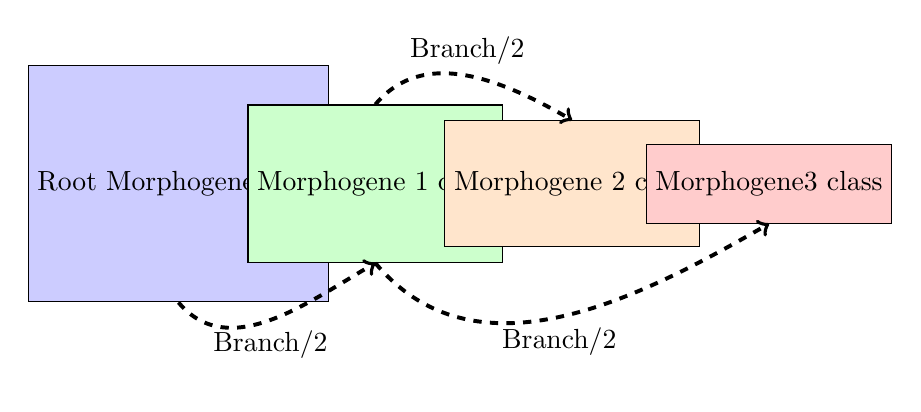
\begin{tikzpicture}
   \foreach \c/\i/\t [count=\n] in  
        {blue!20/Root Morphogene class/1.5,green!20/Morphogene 1 class/1,orange!20/Morphogene 2 class/0.8,red!20/Morphogene3 class/0.5} 
           \node[draw,fill=\c,minimum height=\t * 2cm,minimum width = \t * 1cm,xshift=\n* 2.5cm](N\n){\i} ;
\draw[dashed,->,line width=0.5mm] (N1.south) to [out=-50,in=-150] node[below] {Branch/2} (N2.south);
\draw[dashed,->,line width=0.5mm] (N2.north) to [out=50,in=150] node[above] {Branch/2} (N3.north);
\draw[dashed,->,line width=0.5mm] (N2.south) to [out=-50,in=-150] node[below] {Branch/2} (N4.south);

\end{tikzpicture}
\caption[Possible indirectly encoded genome]{The general structure of the genome (using a subset of the configuration possibilities). The number at the branch denotes the number of child limbs of the following type attached to the respective parent limb.}
\label{figure:genotype}
\end{figure}

\begin{figure}[!h]
\centering
\missingfigure[figwidth=1\textwidth]{Figure of the direct encoding of the genome.}
\caption[Directly encoded genome]{A figure of the direct encoding of the genome.}
\label{figure:direct-encoding}
\end{figure}

\subsubsection{Phenome}
% rev. 2

The Phenomes are the fully developed versions of the genomes. In traditional genetic algorithms, genotypes usually do not have a development stage to transcribe the phenotype from it and be directly evaluated. In modern approaches however, it is often impossible to evaluate the individual directly based on the genotype, especially when the genome structure uses indirect encoding as it is the case in this simulation.
In the Minemonics simulator, two different rigid body constraint models were used to evaluate their stability when used within an evolutionary process. Both phenome models are based on the same representation, but the important difference is the physics simulation model that is used. One of them uses a constrained rigidbody representation reducing the degrees of freedom with constraints, the other uses a Featherstone Multibody representation increasing the degrees of freedom with mobilizers. The main issue which had to be resolved was that the ranges of parameters in the physics engine were not completely clear and some lead to invalid definitions of one or multiple joints, leading to very instable individuals. Instability here means either that a single invalid joint definition leads to instabilities in the solver or that an individual is strained by tensions because the numerical solver is unable to solve multiple contradicting constraints and therefore applies high forces and torques to resolve the constraints even though they can never be resolved. This could be fixed by using the Featherstone Multibody representation as described below. 

\subsubsection{Constrained Rigidbody Phenotype}
% rev. 1

The constrained rigidbody phenotype is build from rigid or softbody primitives and typed joint constraints. Many different joint constraints with different features exist, mainly because some constraints are easier for the solver to handle than others. Generally it is a good strategy to use the most-lightweight constraints over the the computation intensive constrains in order to get a fluid simulation. For the constrained rigidbody phenotype exist many different constraint solvers, the Sequential Impulse Solver (iterative, very bad at large mass ratios), the projected Gauss-Seidel Solver (iterative, bad convergence), and Mixed Linear Complementarity Problem (MLCP) Solvers such as the Dantzig Solver (direct, high computational demand and singularity issues), Lemke Solver (direct, might not converge) or Nonlinear Nonsmooth Conjugate Gradient Solver (iterative, better than PGS, but only at high number of iterations) \cite{bib::Coumans2014}, which results in very stable simulations of complex, hand-made phenotypes. However, problems arise when evolution comes into play, because it evolves and evaluates the whole search space, which results in very diverse individuals and therefore often builds very invalid or strongly contradicting constraint groups. Since in iterative constraint solvers the constraint rows are not solved all at the same time but one after another, the contradicting constraints then apply high forces and torques to the single rigid bodies to resolve the invalid constraint or contradicting constraints, leading to pseudoforces that produce unrealistic physics movement. Therefore the Constraint Rigidbody Phenotype was abandoned and the Featherstone Multibody Phenotype was developed. It might be that using a more constraining genotype representation would lead to only valid and non-contradicting constraints, but such a representation could not be found during the time of this thesis. A more in-depth discussion of the different solvers can be found in \cite{bib::Coumans2014}.

\subsubsection{Featherstone Multibody Phenotype}

The Featherstone Multibody Phenotype is based on the totally different concept of reduced coordinates or generalized coordinates. The reduced coordinates express only the degrees of freedom, starting from the situation where each joint connecting two rigid bodies does not have any DoFs. A simple hinge joint is then expressed as a 1-DoF revolute joint angle. Instead of constraints as in the Constrained Rigidbody Phenotype, we call such a multibody joint a mobilizer. When dealing with maximal coordinates as in all other solvers above, we deal with rigid bodies and pairwise constraints. In that case, we solve the constraints, get the change in velocity for each body and then we compute the velocity and position update individually. In the case of reduced coordinates, the position, velocity and acceleration are expression with reference to the parent limb, meaning that we start at the root element and continue into the child limbs. We also calculate the inertia of the whole hierarchy instead of having only the inertias of the interacting limbs when resolving limb-pairs. In the featherstone representation, it is not necessary to resolve constraints and therefore we do not experience resolving forces and torques, therefore no gaps exist between the rigidbodies. The featherstone representation can not deal with circular structures \cite{bib::Coumans2014}, but such a feature was not needed in this simulation. This phenotype is very robust when it comes to hand-made as well as evolved phenotypes and therefore is much more suitable for evolving virtual creatures. 

\subsubsection{Model organisms}

The model organisms are hand-coded genotypes to be developed into creatures that have specific properties. They are mainly used for testing and experimentation purposes, because they feature a non-redundant, simple genomic description and well defined limb and joint descriptors.

\paragraph{Model Leg}

The model leg is a simple creature built from two equal limbs and one joint. The joint can be either set to be a one DoF hinge joint or a three DoF spherical joint. Its main purpose is to run experiments on chaotic controllers on a simple creature to observe the controller's behavior when controlling a single degree of freedom of a physical system in gravity-less space and on flat-terrain to see the effect of gravity, restitution and friction applied.

\begin{figure}[!h]
\centering
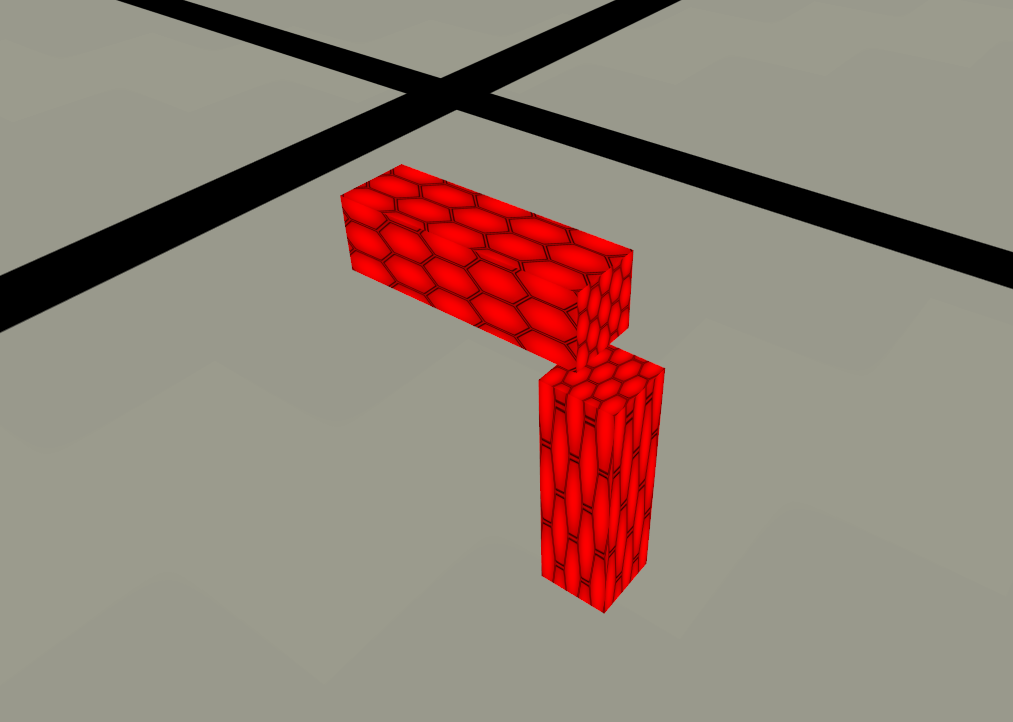
\includegraphics[width=0.32\textwidth]{model-organisms/Model-leg1.png}
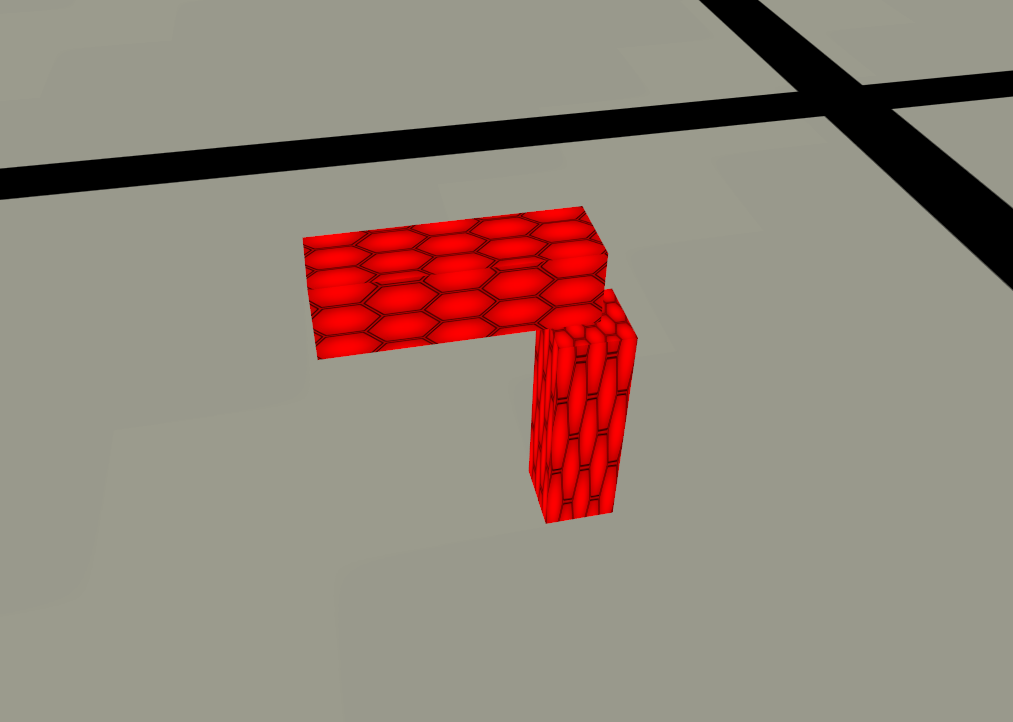
\includegraphics[width=0.32\textwidth]{model-organisms/Model-leg2.png}
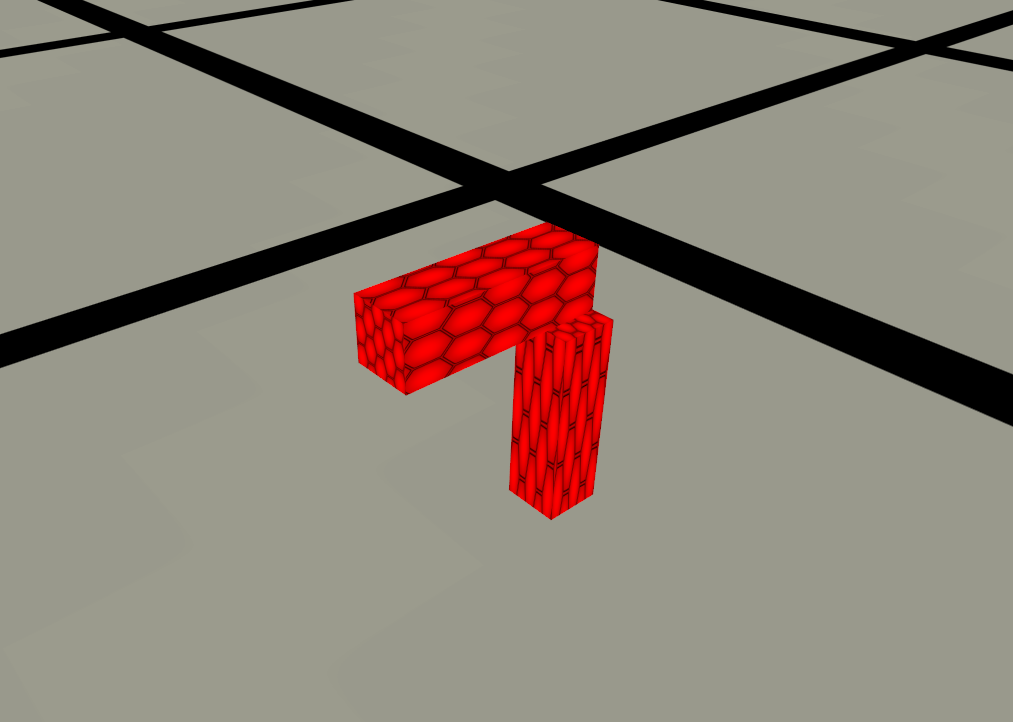
\includegraphics[width=0.32\textwidth]{model-organisms/Model-leg3.png}
\caption[The model leg]{The model leg}
\label{figure:model-leg}
\end{figure}

\paragraph{Snake}

The snake is a creature built from a chain of equal limbs connected with one or three DoF joints as in the case of the model leg. In fact, the snake is just a chain of model legs with a higher number of limb-joint repetitions.

\begin{figure}[!h]
\centering
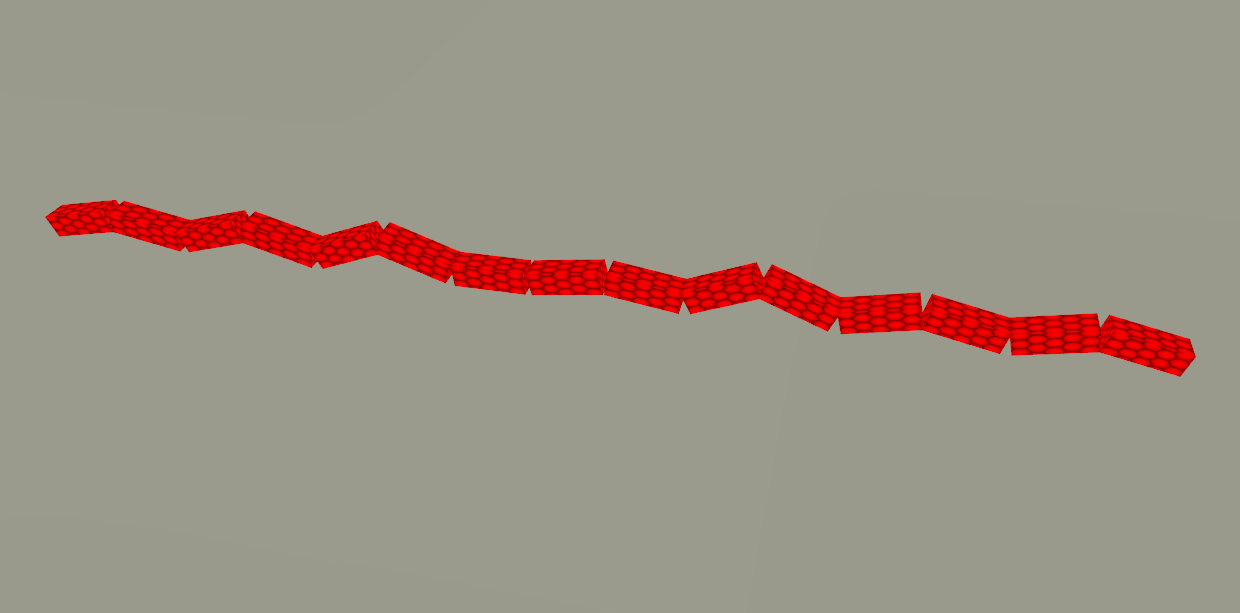
\includegraphics[width=0.32\textwidth]{model-organisms/Model-snake1.png}
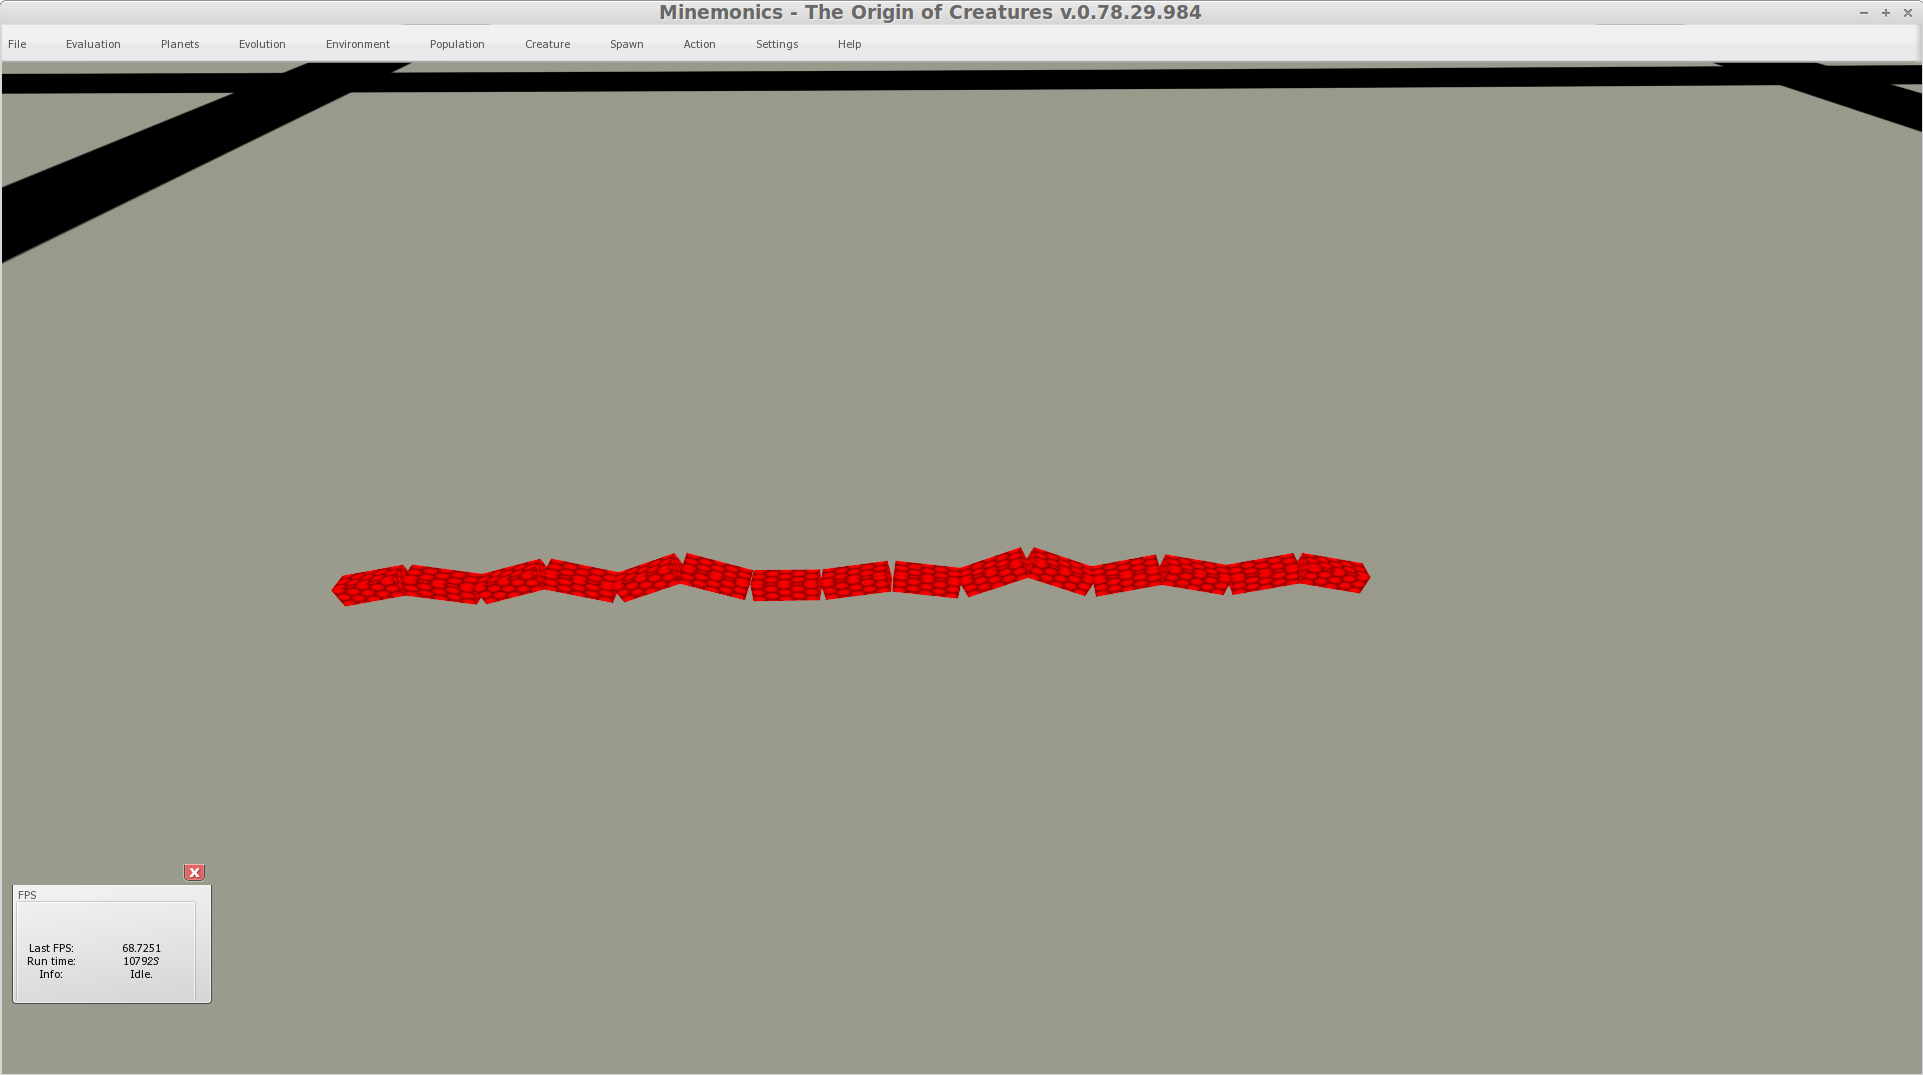
\includegraphics[width=0.32\textwidth]{model-organisms/Model-snake2.png}
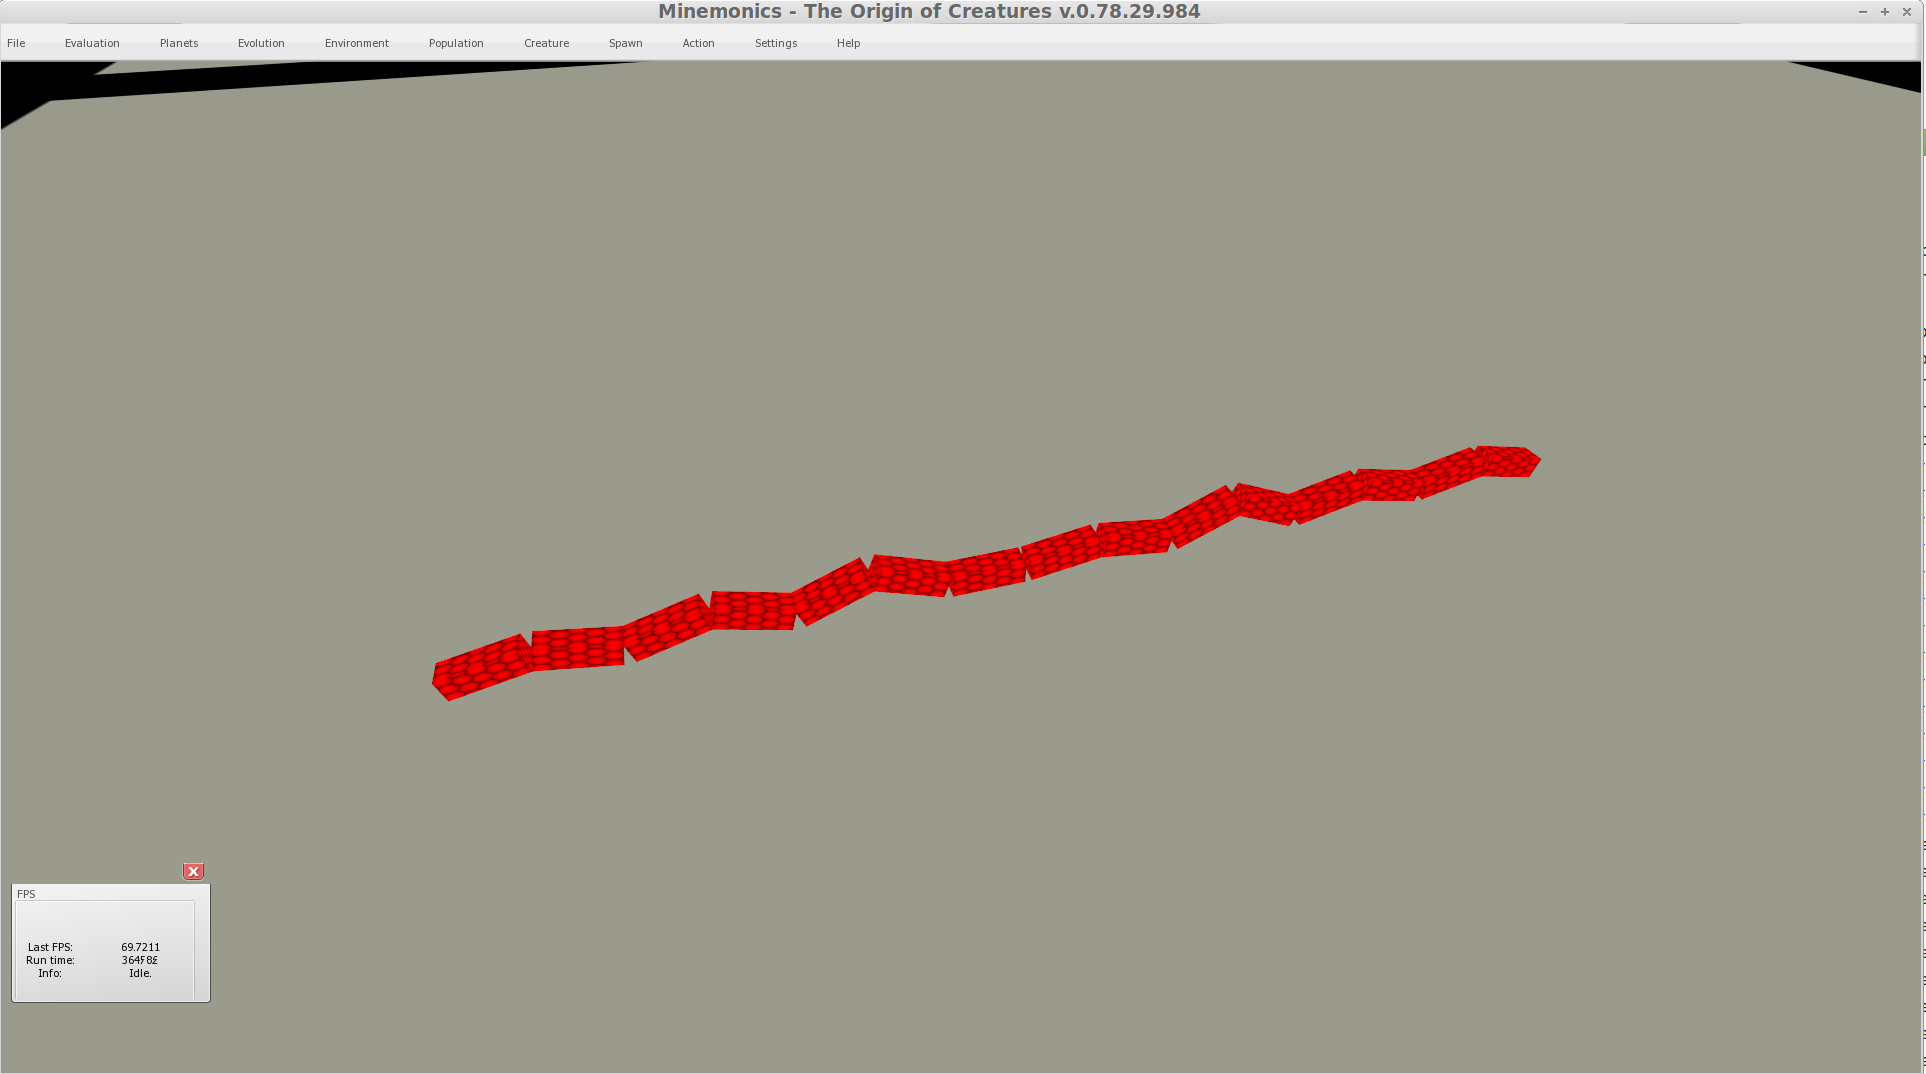
\includegraphics[width=0.32\textwidth]{model-organisms/Model-snake3.png}
\caption[The snake]{The snake}
\label{figure:snake}
\end{figure}

\todo[inline]{Describe the snake model organism.}

\paragraph{Pod}

The Pod is a creature that can be configured to have a certain number of legs and a certain number of body elements. The body is a limb on which the legs are attached in a circular manner. The number of legs is divided by the number of bodies so that the same number of legs is attached to each body. Which the same definition, its is possible to build insect-like creatures such as bugs, spiders, caterpillars and centipedes. It is mainly used to debug the Genotype-to-Phenotype transcription (Embryogenesis).

\begin{figure}[!h]
\centering
\missingfigure[figwidth=1\textwidth]{Figure of the pod model organism.}
\caption[The pod]{The pod}
\label{figure:pod}
\end{figure}

\todo[inline]{Describe the pod model organism.}

\paragraph{Ragdoll}

The ragdoll blueprint produces a human-like form. It consists of differently configured joints and is mainly used to debug the Genotype-to-Phenotype transcription (Embryogenesis).

\begin{figure}[!h]
\centering
\missingfigure[figwidth=1\textwidth]{Figure of the ragdoll model organism.}
\caption[The ragdoll]{The ragdoll}
\label{figure:ragdoll}
\end{figure}

\todo[inline]{Describe the ragdoll model organism.}

\subsection{Embryogenesis}

\begin{figure}[!h]
\centering
\missingfigure[figwidth=1\textwidth]{Add a figure of the embryogenesis processing}
\caption[Structure of the embryogenesis]{Structure of the embryogenesis}
\label{figure:embryogenesis}
\end{figure}

The embryogenesis of a creature is a straight-forward process transcribing a genotype into a phenotype. Starting from the root morphogene, the genome is expanded in a breath-first-search manner. This means that it starts at the root node and expands its child nodes first, before moving on to the higher degree children. The embryogenesis is performed using phenotype generators. Phenotype generators help to keep some intermediate results in the generation process, namely the morphogene branch of the parent morphogene and the parent limb element, the position and orientation of the current generation, the current shrinkage factor of the generated limbs, if this is a flipped or mirrored branch, the length of the current root to leaf path and a list of the number of repetitions of different morphogene classes along this branch.  To setup the embryogenesis so that the same processing can be done for every morphogene, the root morphogene is assigned to a Phenotype generator and inserted into an empty list of generators. The phenotype generator's base orientation is initialized to the quaternion identity, the segments depth limit and the total segments quantity is set to 0 and the repetition lists are emptied. Then the processing of a morphogene and its morphogene branches works as follows: we take the first generator out of the list, then we check if we reached the total segment limit or the segments depth limit defined by the individual. If it is reached, the phenotype is finished, else we continue. Now we create the new limb according to the morphogene specifications. Then we check if this limb has to be appended to a existing parent limb (for the root morphogene no, for all others yes), if yes, we position the child limb so that their joint anchoring points on the surface of both limbs overlap, then we connect them by defining the joint as defined in morphogene branch connecting the two limbs. Finally we produce the new generators and insert them into our generator list, one for each morphogene branch of the child morphogene we just processed. 

\subsection{Reaper}
\label{subsection:Reaper}

At the end of all evaluations for a certain generation of a population, the simulation arrives at the evolution step.  In the evolution step, the following operations are performed by the reaper: Culling a percentage of the worst performing creatures according to the total fitness ranking, variation of the remaining creatures with different variance operators according to the respective percentages and sowing of new creatures partly from crossover and random generation. In the Minemonics simulator, the following percentages were chosen:

\begin{itemize}
\item Reap percentage: \unit[15]{\%}
\item Variation on the rest of the population (considered \unit[100]{\%} in the following list)
\begin{itemize}
\item Elitism (no variation): \unit[16.6]{\%}
\item Gene specification mutation percentage: \unit[16.6]{\%}
\item Gene split percentage: \unit[16.6]{\%}
\item Branch mutation percentage: \unit[16.6]{\%}
\item Grow stub gene percentage: \unit[16.6]{\%}
\item Graft feature percentage: \unit[16.6]{\%}
\end{itemize}
\item Sow percentage: \unit[15]{\%}
\begin{itemize}
\item Crossover: \unit[50]{\%}
\item Random generation: \unit[50]{\%}
\end{itemize}
\label{item:ReaperPerc}
\end{itemize}

In the following sections, the different operations are described in detail.

\subsubsection{Culling}
\label{subsubsection:Culling}

In order to cull individuals from the population, the individuals first have to be sorted according to their fitness. For a single fitness function, the sorting is straight forward. But in many cases, it is necessary to have individuals adapt to multiple fitness functions to represent the desired fitness landscape. Furthermore it might be, that one of the fitness functions should have a higher weight than the others. To combine the different fitness functions is hard, usually because it is not possible to adjust them to the same scaling, especially when one of them is the better the lower its value is. Therefore, competitive ranking was chosen to combine the fitness functions. This means that for each fitness function, we sort the individuals according to their respective fitness value and assign a number of points to each rank (in the simulator, the number of points for a rank is the number of individuals that performed worse). Then we sum for each individual $c_n$ for $m$ fitness functions, the ranking points $r_i$ multiplied by the respective fitness function weight $w_i$. 

\[\text{fitness score}_{c_n} = \sum\limits^m_{i=1} r_i \cdot w_i \]

Finally, we sort the individuals by their fitness score, which gives us their total ranking according to their fitness. Unfortunately, by this procedure, the score loses the information whether the best individual of the creature increased its fitness. However this can easily be found out by printing out all fitness function values of the best creature of the population at the end of the evaluation.

\subsubsection{Crossover}
\label{subsec:crossover}

The typical crossover strategy inspired by biological crossover is commonly known as cutting the two parent genomes into segments and then recombining segments of the parents into a new valid genome. This section additionally describes the procedure on how to choose matching parents.

Using the creatures sorted by the fitness ranking, a percentage of those best performing creatures (based on list \ref{item:ReaperPerc}) are chosen to be possible parents. To create the new offsprings, we iterate over all possible parents, taking every possible parent for the number of offsprings per parent (the number of offsprings per parent is found by diving the total number of new creatures created by crossover by the number of parents). Having found one of the parent, the other parent is chosen as follows: With \(\unit[50]{\%}\) chance, the parent is chosen as one from a tournament of 10, where the best creature of that tournament is chosen as the second partner. Each tournament creature is drawn from the population using a normal positive integer distribution such that the \(\mu\) is on the index of the first creature and the \(\sigma\) is such that the probability decays nearly completely until the index of the last creature. Additionally, the distribution is capped to output the index of the last creature at maximum. With the remaining \(\unit[50]{\%}\) chance, the second parent is chosen at random from the population.

The actual crossover process is very similar to the commonly known one. A subsegment is taken of each genome of the parents and the two segments are then combined. Different from the process in classical bit-array notions of genomes is that the two segments have to be interconnected with branches in order to be properly combined. Therefore we mutate 10 random branches and repair all the gene branches to have valid branching indices again.

\subsubsection{Mutations}

The other variational operators all work on single elements of a single genome except for the graft feature mutation. The mutations modify specific aspects of the genome and are specifically made for the genomic structure.

\paragraph{Gene specification mutation}

The gene specification mutation applied to a genome iterates over all its morphogene classes. For each class, with probability $0.2$, the morphogene is reinitialized with random values. This affects all values except for the morphogene branches which stay unchanged.

\paragraph{Gene split mutation}

The gene split mutation applied to a genome iterates over all morphogene classes. For each class, with probability $0.2$, the morphogene is split along the X, Y or Z axis into two morphogenes occupying roughly the same total volume as the original limb. The morphogenes are then connected with a single branch.

\paragraph{Branch specification mutation}

The branch specification mutation applied to a genome iterates over all morphogene classes. For each class, with probability $0.2$, a random morphogene branch is chosen and is reinitialized with random values. 

\paragraph{Grow stub gene mutation}

The grow stub gene mutation applied to a genome iterates over all morphogene classes. For each class, with probability $0.6$, $x$ new branches are added to the morphogene, where $x \in [0,2]$. The branches reconnect the stub gene to others and therefore increase the interconnectivity of unconnected morphogene classes.

\paragraph{Graft feature mutation}

The graft feature mutation is similar to crossover, but instead of just cutting both genomes at random positions and recombining them, it picks a random morphogene in the donor genome and copies this morphogene and its children over to the receiver genome until copying depth $x$ is reached, where $x \in [5,10]$. As the name says, the idea of this mutation would be to copy a segment functionally to move a random feature from one creature to another. By this mutation, a limb configuration producing a specific structure could be transferred.

\section{Evolutionary cycle}
% rev. 1

To describe how the different components play together, an evolutionary cycle of one planet with a flat plane environment and a population of 10 individuals is outlined. One evolutionary cycle can be separated into 2 substeps, the evaluation step and the variation step. Before the cycle can begin, the planet and its environment is set up, the (infinite) flat plane is positioned at the origin of the coordinate system, and each randomly generated individual's genome is transcribed into a phenotype by the embryogenesis. The population is not yet visible anywhere and awaits evaluation.

\subsection{Evaluation step}
% rev. 1

During the evaluation step, each individual is dropped into the simulation slightly above the ground for the selected evaluation period of usually 20 seconds. In single creature mode which was used for all experiments, every creature is evaluated separately and the controller starts to move the limbs. If a creature consists of 0 or only 1 limb, the creature is discarded, since it is degenerate and can not move at all, therefore it is worthless to evaluate it. Furthermore, the evolution discards creatures that produce very high joint velocities, which is usually an indication that the creature might exploit unrealistic physical forces. During the evaluation of the other creatures, the juries evaluate the performance and calculate the combined fitness value at the end of the evaluation. If all evaluations are over, the evolution switches to the variation step.

\subsection{Variation step}
% rev. 1

During the variation step, the reaper picks up the population, culls the worst performing creatures, leaves a top percentage of creatures without variation (Elitism), instead produces offspring by crossover based on them and an additional partner, then applies the mutations to the rest of the population according to list \ref{item:ReaperPerc} and finally replaces the missing number of creatures with new, randomly generated creatures.

\end{document}